\section{Proprietà di stabilità di un sistema LTI}
Se abbiamo un sistema LTI (Lineare tempo invariante) rappresentato da una
funzione di trasferimento $H(s)$, sappiamo che la sua uscita $y(t)$ è data da:
\begin{equation}
    y(t) = \mathbb{L}^{-1}\{C(SI -A)^{-1} + x(\phi)\}+ \mathbb{L}^{-1}\{[C(SI -A)^{-1}B + D]U(s)\}
\end{equation}

dove il primo termine rappresenta la risposta libera del sistema (ovvero la
risposta dovuta alle condizioni iniziali) e il secondo termine rappresenta la
risposta forzata (ovvero la risposta dovuta all'ingresso $u(t)$). Essendo un
sistema asintoticamente stabile, la risposta libera tende a zero nel tempo,
mentre la risposta forzata dipende dall'ingresso $u(t)$ e dalla funzione di
trasferimento $H(s)$. Adesso ci interessa la BIBO stabilità perché ci stiamo
riferendo alla risposta forzata. Ognuno di questi tratti semplici dà un
contributo alla risposta. In particolare, tutti i termini che nascono dai poli
della funzione di trasferimento sono chiamati modi naturali del sistema, e la
loro stabilità dipende dalla posizione dei poli nel piano complesso. Gli altri
modi sono chiamati modi forzati (modi di ingresso) e dipendono dall'ingresso
$u(t)$ e dalla funzione di trasferimento $H(s)$. Andando a scomporre
ulteriormente la risposta forzata, possiamo identificare i contributi dei modi
naturali e dei modi forzati. Abbiamo quindi che la risposta complessiva del
sistema è data da:
\begin{equation}
    y(t) = y_{zi}(t) + y_{tr}(t) + y_{ss}(t)
\end{equation}
In particolare sappiamo che la somma tra $y_{zi}(t)$ e $y_{tr}(t)$ quando $t$ tende a infinito tende a zero; questa si chiama risposta transitoria, mentre $y_{ss}(t)$ è la risposta in regime permanente.
La risposta trasitoria e la risposta in regime permanente sono definite se e solo se siamo in uno dei seguenti casi:
\begin{enumerate}
    \item Il sistema è asintoticamente stabile;
    \item Il sistema è BIBO stabile e le condizioni iniziali sono nulle.
\end{enumerate}

\subsection{Risposta stato stabile}
Come abbiamo detto, la risposta in regime permanente è data da $y_{ss}(t)$.
\begin{tcolorbox}[title=Esempio funzione a gradino]
    Vogliamo calcolare la risposta in regime permanente di un sistema BIBO stabile a fronte di un segnale a gradino.
    Avremo quindi:
    \begin{itemize}
        \item H(s) BIBO stabile;
        \item $u(t) = U \cdot \epsilon(t)$, dove $\epsilon(t)$ è la funzione a gradino unitario.
        \item calcolare $y_{ss}(t)$.
    \end{itemize}
    Per calcolare la risposta in regime permanente, possiamo utilizzare il teorema del valore finale, che afferma che se $H(s)$ è BIBO stabile, allora:
    \begin{equation}
        \lim_{t \to \infty} y(t) = \lim_{s \to 0} sY(s)
    \end{equation}
    Procedo a calcolare questo limite come:
    \begin{equation}
        \lim_{s \to 0} sY(s) = \lim_{s \to 0} sH(s)U(s)
    \end{equation}
    Sostituendo $U(s)$ con la trasformata di Laplace del segnale a gradino, otteniamo:
    \begin{equation}
        \lim_{s \to 0} sH(s) \cdot \frac{U}{s} = U \cdot \lim_{s \to 0} H(s)
    \end{equation}
    Essendo $H(s)$ BIBO stabile, al denominatore non ho poli a $s=0$, quindi posso calcolare il limite sostituendo $s$ con $0$:
    \begin{equation}
        U \cdot H(0)
    \end{equation}
    Quindi la risposta in regime permanente a fronte di un segnale a gradino è data da $U \cdot H(0)$.
\end{tcolorbox}
\begin{tcolorbox}[title=Esempio funzione sinusoidale]
    Vogliamo calcolare la risposta in regime permanente di un sistema BIBO stabile a fronte di un segnale sinusoidale.
    Avremo quindi:
    \begin{itemize}
        \item H(s) BIBO stabile;
        \item $u(t) = U \cdot \sin(\omega t)$, dove $\omega$ è la frequenza del segnale sinusoidale.
        \item calcolare $y_{ss}(t)$.
    \end{itemize}
    La mia $y_{ss}(t)$ sarà data da:
    \begin{equation}
        y_{ss}(t) = \bar{y}(\omega_0)sin(\omega_0 t + \phi(\omega_0)) \rightarrow \bar{y}(\omega_0) = |H(j\omega_0)| \cdot U, \quad \phi(\omega_0) = \arg(H(j\omega_0))
    \end{equation}
    Abbiamo dai dati del problema che:
    \begin{itemize}
        \item $H(s) = \frac{1}{(s+2)(s+10)}$
        \item $u(t) = 2 sin(0.5t)\epsilon(t)$
    \end{itemize}
    Sostituendo i dati del problema nella formula della risposta in regime permanente, otteniamo:
    \begin{equation}
        y_{ss}(t) = \bar{y}(0.5)sin(0.5t + \phi(0.5)) \rightarrow \bar{y}(0.5) = |H(j0.5)| \cdot 2, \quad \phi(0.5) = \arg(H(j0.5))
    \end{equation}

    Proviamo a calcolare questo in MATLAB:
    \begin{verbatim}
        s = tf('s');
        H = 1/((s+2)*(s+10));
        w0 = 0.5;
        [m,f] = bode(H,w0);

        f_rad = f/180*pi; % Converti da gradi a radianti

    \end{verbatim}
    Otteniamo che \verb|m = 0.0484|, \verb|f = -16.8986| e quindi
    \verb|f_rad = -0.2949|. Sostituendo questi valori nella formula della risposta
    in regime permanente, otteniamo:
    \begin{equation}
        y_{ss}(t) = 0.0968sin(0.5t - 0.2949)
    \end{equation}

\end{tcolorbox}
La funzione $H(j\omega)$ è chiamata funzione di risposta in frequenza del sistema, e ci permette di capire come il sistema risponde a segnali sinusoidali di diversa frequenza. In particolare, la magnitudine $|H(j\omega)|$ ci dice quanto il sistema amplifica o attenua un segnale sinusoidale di frequenza $\omega$, mentre la fase $\arg(H(j\omega))$ ci dice quanto il sistema ritarda o anticipa un segnale sinusoidale di frequenza $\omega$.
\begin{center}
    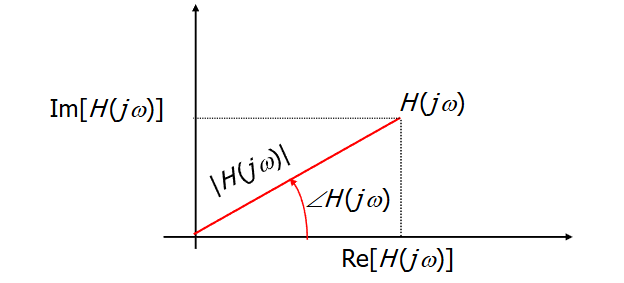
\includegraphics[scale=0.5]{foto/cph5/1.png}
\end{center}
$H(j\omega)$ si può rappresentare in diverse forme:
\begin{itemize}
    \item forma cartesiana: $H(j\omega) = Re(H(j\omega)) + jIm(H(j\omega))$
    \item forma polare: $H(j\omega) = |H(j\omega)|e^{j\arg(H(j\omega))}$
    \item diagramma di Bode: rappresentazione della magnitudine e della fase in funzione
          della frequenza $\omega$ su scala logaritmica.
\end{itemize}

\subsection{Rappresentazioni}
\subsubsection{Diagramma di Bode}
I diagrammi di Bode sono rappresentazioni grafiche della risposta in frequenza
di un sistema. Il diagramma di Bode è composto da due grafici: il primo
rappresenta la magnitudine $|H(j\omega)|$ in decibel (dB) in funzione della
frequenza $\omega$ su scala logaritmica, mentre il secondo rappresenta la fase
$\arg(H(j\omega))$ in gradi in funzione della frequenza $\omega$ su scala
logaritmica.
\begin{center}
    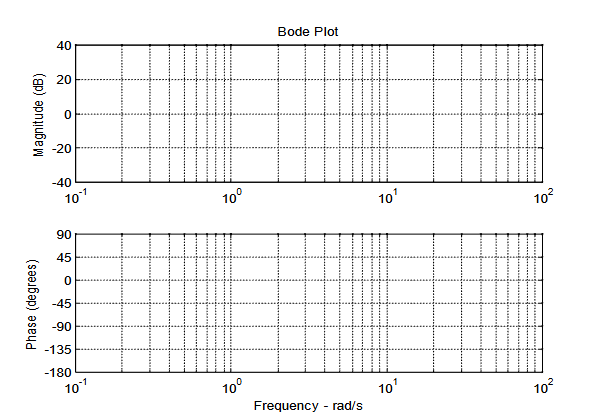
\includegraphics[scale=0.5]{foto/cph5/2.png}
\end{center}

Per calcolare il diagramma devo usare la dc-form della funzione di
trasferimento, che è data da:
\begin{equation}
    H(s) = K \cdot \frac{(s-z_1)(s-z_2)...(s-z_m)}{(s-p_1)(s-p_2)...(s-p_n)}
\end{equation}

\begin{tcolorbox}
    Ipotizziamo di avere una funzione di trasferimento del tipo:
    \begin{equation}
        H(s) = 10\frac{1+\frac{s}{2}}{s(1+s+s^2)}
    \end{equation}
    Per calcolare il diagramma di Bode, calcolo prima la magnitudine $|H(j\omega)|$ e la fase $\arg(H(j\omega))$:
    \begin{equation}
        |H(j\omega)| = 20 log_{10}(|H(j\omega)|) =
    \end{equation}
\end{tcolorbox}

\newpage
\begin{minipage}{0.45\linewidth}
    \begin{center}
        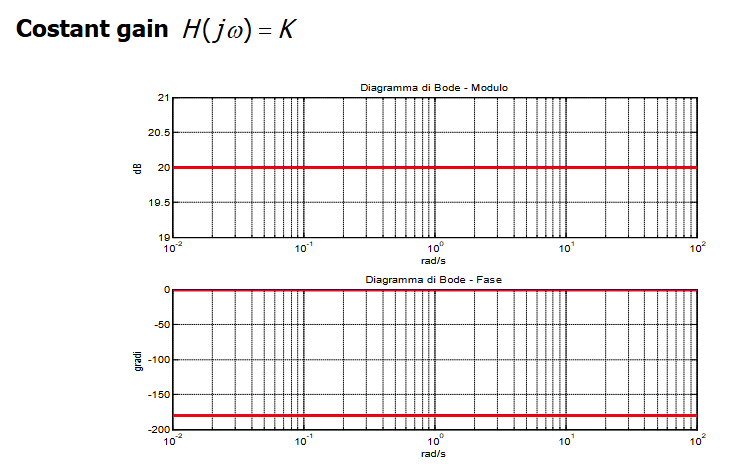
\includegraphics[scale=0.5]{foto/cph5/3.png}
    \end{center}
\end{minipage}
\begin{minipage}{0.45\linewidth}
    \begin{center}
        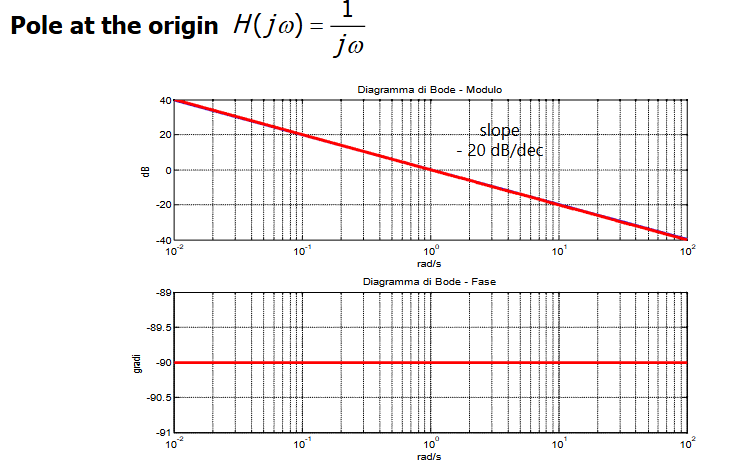
\includegraphics[scale=0.5]{foto/cph5/4.png}
    \end{center}
\end{minipage}
\newline
\begin{minipage}{0.45\linewidth}
    \begin{center}
        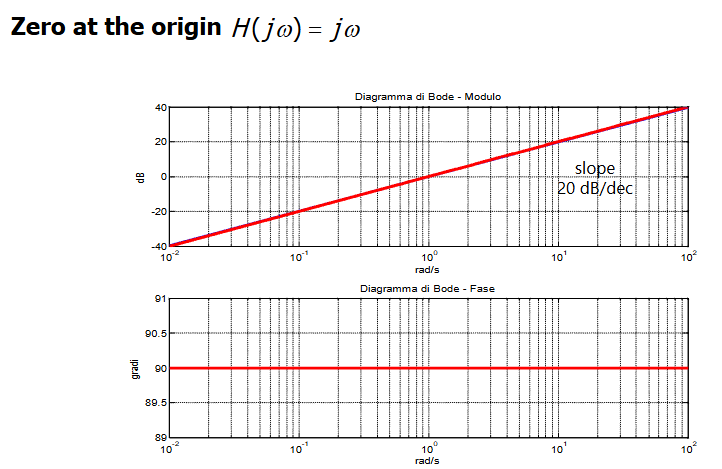
\includegraphics[scale=0.5]{foto/cph5/5.png}
    \end{center}

\end{minipage}
\begin{minipage}{0.45\linewidth}
    \begin{center}
        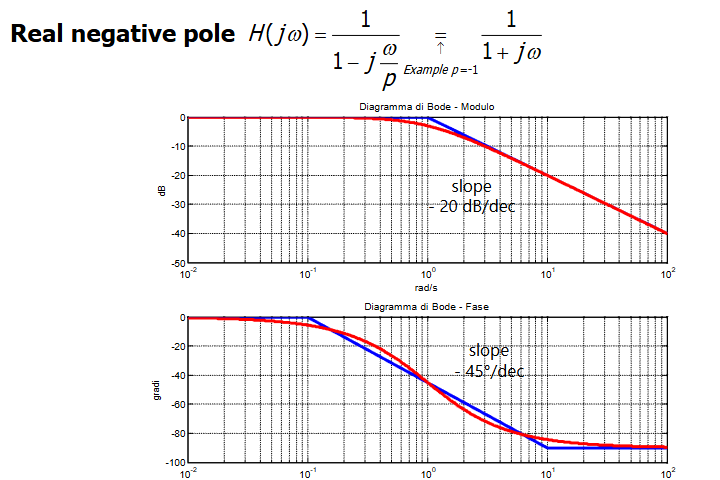
\includegraphics[scale=0.5]{foto/cph5/6.png}
    \end{center}
\end{minipage}
\newline
\begin{minipage}
    {0.45\linewidth}
    \begin{center}
        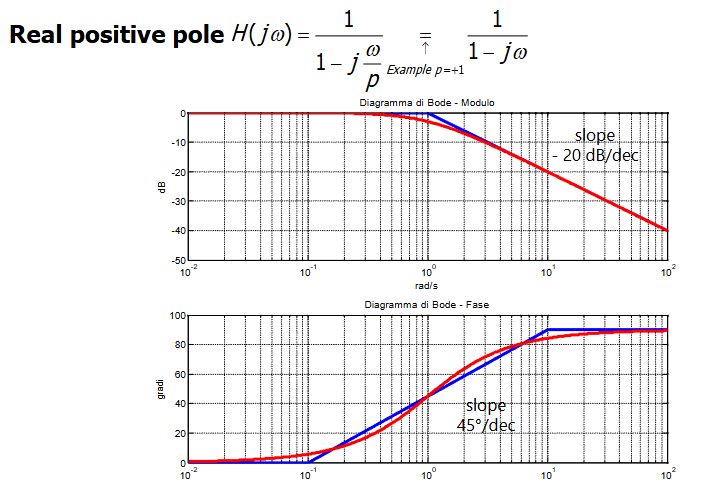
\includegraphics[scale=0.5]{foto/cph5/7.png}
    \end{center}
\end{minipage}
\begin{minipage}{0.45\linewidth}
    \begin{center}
        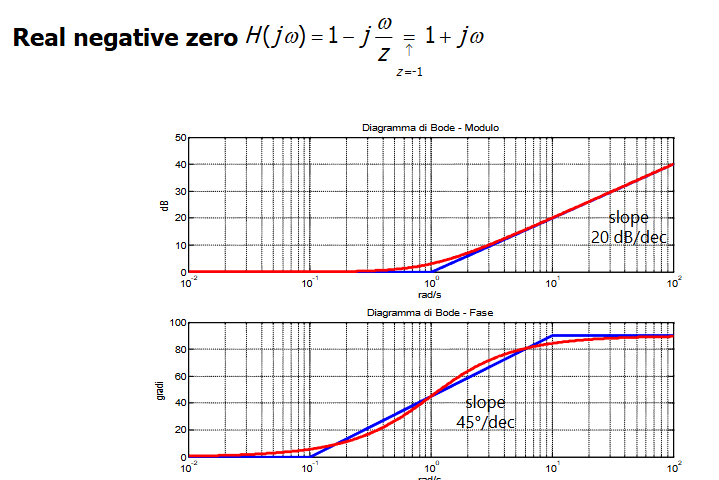
\includegraphics[scale=0.5]{foto/cph5/8.png}
    \end{center}
\end{minipage}
\newline
\begin{minipage}
    {0.45\linewidth}
    \begin{center}
        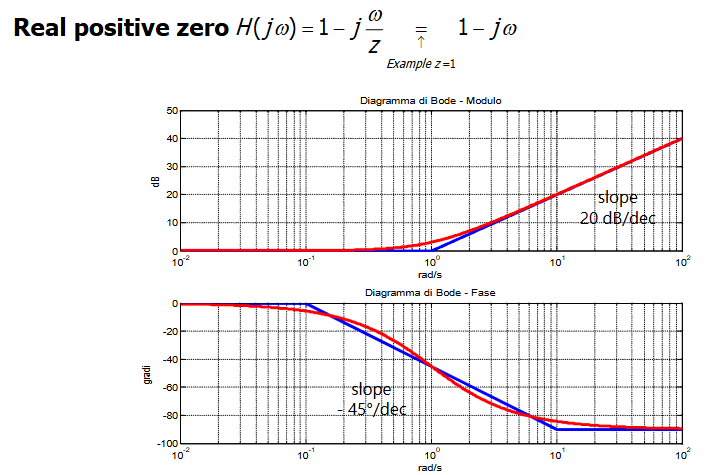
\includegraphics[scale=0.5]{foto/cph5/9.png}
    \end{center}
\end{minipage}
\begin{minipage}{0.45\linewidth}
    \begin{center}
        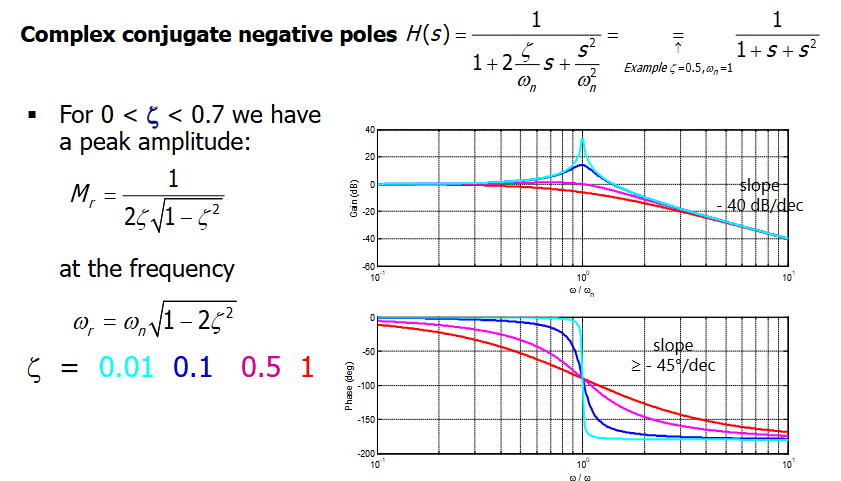
\includegraphics[scale=0.4]{foto/cph5/10.png}
    \end{center}
\end{minipage}
\newline
\begin{minipage}
    {0.45\linewidth}
    \begin{center}
        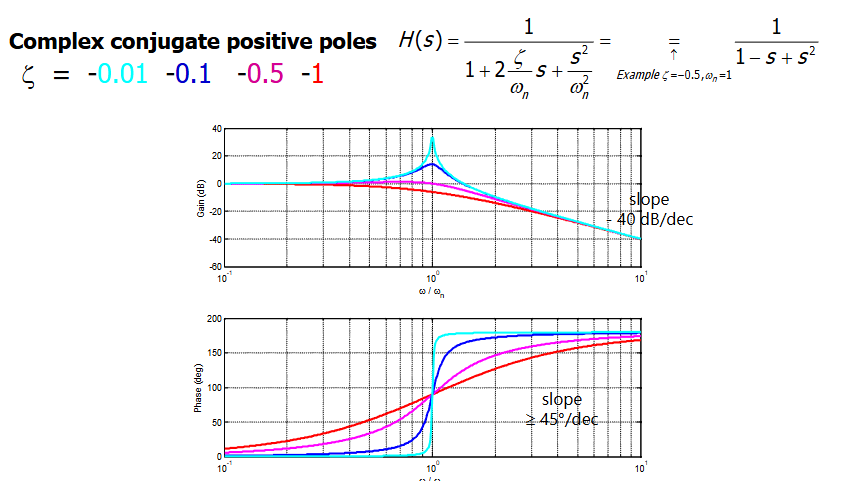
\includegraphics[scale=0.4]{foto/cph5/11.png}
    \end{center}
\end{minipage}
\hfill
\begin{minipage}{0.45\linewidth}
    \begin{center}
        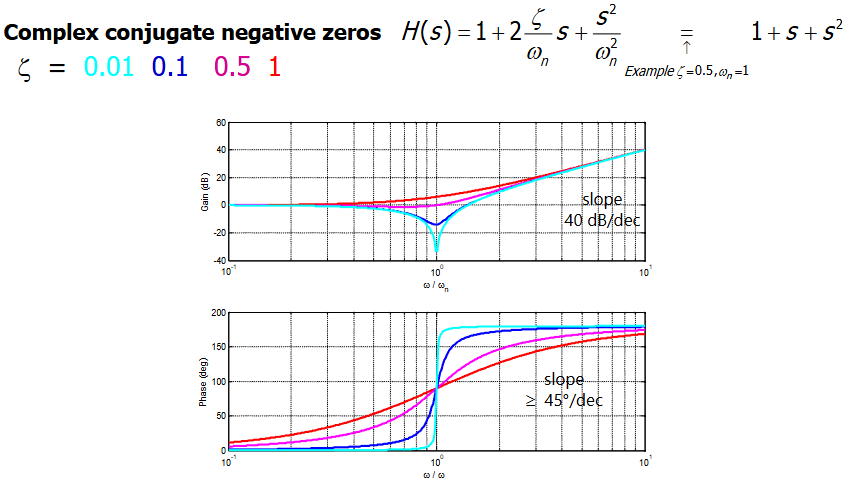
\includegraphics[scale=0.4]{foto/cph5/12.png}
    \end{center}
\end{minipage}
\newline
\begin{minipage}
    {0.45\linewidth}
    \begin{center}
        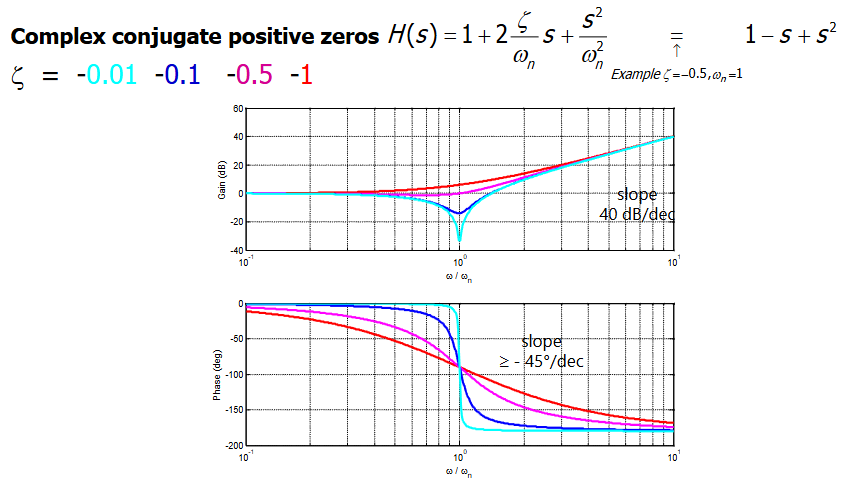
\includegraphics[scale=0.4]{foto/cph5/13.png}
    \end{center}
\end{minipage}

In MATLAB, possiamo utilizzare la funzione \verb|bode| per calcolare il
diagramma di Bode di una funzione di trasferimento. Ad esempio, se abbiamo la
funzione di trasferimento $H(s) = \frac{1}{(s^2 +3*s+2)}$, possiamo calcolare
il diagramma di Bode con il seguente codice:
\begin{verbatim}
    s = tf('s');
    H = 1/(s^2 +3*s+2);
    figure, bode(H);
\end{verbatim}
Questo codice creerà un grafico con la magnitudine e la fase di $H(j\omega)$ in
funzione della frequenza $\omega$ su scala logaritmica. Se faccio
\verb|omega = logspace(a,b,n)|, ottengo un vettore di $n$ punti equispaziati in
scala logaritmica tra $10^a$ e $10^b$. Se voglio calcolare il diagramma di Bode
in un intervallo di frequenze $\omega$ specifico, posso usare
\verb|bode(H,omega)|. Il comando Bode non sempre restituisce un grafico
conveniente per l'uso che ci serve.

\subsubsection{Diagramma polare}
Un diagramma polare è una rappresentazione grafica della risposta in frequenza
ottenuta rappresentando la parte immaginaria $Im[H(j\omega)]$ in funzione della
parte reale $Re[H(j\omega)]$ in un singolo piano parametrizzato ed orientato in
$\omega$. Ogni grafico corrisponde ad un valore di frequenza $\omega$. Un
approssimazione del diagramma polare può essere ottenuta a partire dal
diagramma di Bode, utilizzando le seguenti relazioni:
\begin{equation}
    Re[H(j\omega)] = |H(j\omega)| \cdot \cos(\arg(H(j\omega)))
\end{equation}
\begin{equation}
    Im[H(j\omega)] = |H(j\omega)| \cdot \sin(\arg(H(j\omega)))
\end{equation}
Per usare il diagramma polare su MATLAB, possiamo utilizzare la funzione \verb|nyquist|. Ad esempio, se abbiamo la funzione di trasferimento $H(s) = \frac{1}{(s^2 +3*s+2)}$, possiamo calcolare il diagramma polare con il seguente codice:
\begin{verbatim}
    s = tf('s');
    H = 1/(s^2 +3*s+2);
    [re, im] = nyquist(H);
    figure, plot(squeeze(re), squeeze(im));
\end{verbatim}
La funzione \verb|nyquist| restituisce due array, uno per la parte reale e uno
per la parte immaginaria di $H(j\omega)$; la funzione \verb|squeeze| viene
utilizzata per rimuovere le dimensioni singleton dagli array restituiti da
\verb|nyquist|, in modo da poterli utilizzare direttamente nella funzione
\verb|plot| per tracciare il diagramma polare.
\subsubsection{Diagramma di Nyquist}

\subsubsection{Diagramma di Nichols}
Il diagramma di Nichols è una rappresentazione grafica della risposta in
frequenza ottenuta rappresentando la magnitudine $|H(j\omega)|$ in decibel (dB)
in funzione della fase $\arg(H(j\omega))$ in gradi. Ogni punto del diagramma
corrisponde ad un valore di frequenza $\omega$. Impropriamente, possiamo dire
che il diagramma di Nichols è la fusione dei diagrammi di Bode, in cui la
magnitudine e la fase sono rappresentate nello stesso grafico.